%%%%%%%%%%%%%%%%%%%%%%%%%%%%%%%%%%%%%%%%%%%%%%%%%%%%%%%%%%%%%%%
%CRONOGRAMA
%%%%%%%%%%%%%%%%%%%%%%%%%%%%%%%%%%%%%%%%%%%%%%%%%%%%%%%%%%%%%%%

\chapter{Cronograma}

\begin{table}[h]
\centering
\makebox[\textwidth][c]{%
\setlength{\tabcolsep}{8pt}
\begin{tabular}{|l|c|c|c|c|c|}
\hline
\rowcolor[HTML]{A7D3E9}
\textbf{2026.1} & \textbf{Fevereiro} & \textbf{Março} & \textbf{Abril} & \textbf{Maio} & \textbf{Junho} \\
\hline

\rowcolor[HTML]{D6EBF5}
Correção da Elaboração de Projeto
&  &  &  &  &  \\
\hline

\rowcolor[HTML]{FFFFFF}
Desenvolvimento da Documentação de Software 
&  &  &  &  &  \\
\hline

\rowcolor[HTML]{D6EBF5}
Desenvolvimento Frontend 
&  &  &  &  &  \\
\hline

\rowcolor[HTML]{FFFFFF}
Desenvolvimento Backend
&  &  &  &  &  \\
\hline

\rowcolor[HTML]{D6EBF5}
Elaboração EPP -- Metodologia 
&  &  &  &  &  \\
\hline

\end{tabular}
}
\caption{Cronograma de atividades do projeto} 
\label{tab:cronograma}
\end{table}

\begin{comment}
\begin{figure}[H]
	\begin{center}
	    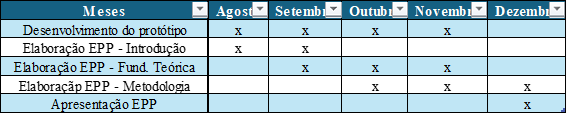
\includegraphics[scale=1.0]{imagens/cronograma-epp.png}
	\end{center}
    \caption{\label{fig_arranjo}Cronograma.}
	\legend{Fonte: Elaborado pelo Autor}
    \label{fig:cronograma}
\end{figure}
\end{comment}
